\documentclass[a4paper,12pt]{article} 
\usepackage[spanish]{babel}	%Escritura con acentos
\usepackage[utf8]{inputenc} %Codificación UTF-8 
\usepackage{imakeidx}
\usepackage{graphicx}       %Para incluir figuras
\usepackage{float}
\usepackage[backend=bibtex,style=verbose]{biblatex}
\bibliography{bibliography}
\usepackage{csquotes}
\usepackage{tcolorbox}
\begin{document}

\title{Medida de Permeabilidad del Vacío}

\author{Gabriel D'Andrade Furlanetto - XDD204950}

\maketitle
\section{Objetivos}
Se tiene como objetivo principal de la experiencia el cálculo del coeficiente de permeabilidad magnética del vacío, $\mu_0$. Para esto, se han utilizado bobinas cilíndricas de diámetros, longitudes y número de espiras conocidas, 
poniéndolas una adentro de la otra. De esta manera, se introduce una corriente alterna en la bobina principal con un oscilador y se mide el voltaje inducido en la bobina secundaria. 

Con esto, se puedo medir indirectamente el coeficiente de inducción mútua, $M_{12}$ y, finalmente, se puede utilizar este resultado para encontrar $\mu_0$.
Este proceso se repite dos veces para comparar los resultados de diferentes bobinas y, finalmente, se hace una medida indirecta de la constancia del campo magnético en la bobina para se saber cuanto se puede justificar las premisas que llevan a las ecuaciones utilizadas.


\section{Material Utilizado}
\begin{itemize}
    \item Bobina 1: $\Phi_1 = 12.5cm \qquad N_1=317 \qquad l_1=50cm$
    \item Bobina 2:  $\Phi_2 = 3.2cm \qquad N_2=190 \qquad l_2=30cm$
    \item Bobina 3:  $\Phi_3 = 5.1cm \qquad N_3=257 \qquad l_3=40cm$
    \item Dos multímetros para medir la intensidad y el voltaje inducido
    \item Un oscilador para regular la frecuencia y la corriente
\end{itemize}
\section{Realización práctica}

\subsection{Cálculo de $\mu_0$ a partir del coeficiente de inducción mutua entre las bobinas 1 Y 2}
El cálculo del coeficiente de permeabilidad magnética del vacío está contingente en una série de ecuaciones que relacionan los datos experimentales obtenidos (esto es, la intensidad, voltaje inducida y la frecuencia) al llamado coeficiente de inductancia mútua, $M_{12}$ y otro par de ecuaciones que lo relacionan a la geometría de las bobinas y el coeficiente de permeabilidad.

De esta manera, la idea fundamental de este apartado es calcular de la manera más precisa posible $M_{12}$ a partir de $I_e$ y $V_e$, haciendo dos regresiones lineales para minimizar las incertidumbres. Empezando por la ecuación

$$V_e = \left(2\pi f \cdot M_{12}  \right)I_e $$

O sea, si se hace una regresión lineal de $V_e$ en función de $I_e$, el valor de la pendiente $k$ será igual a

$$k = \left(  2\pi M_{12}\right) f$$

Por lo tanto, si se hace la regresión anterior para diferentes valores de $f$ y, finalmente, se pone $k$ como función de $f$, la pendiente será igual a $2\pi M_{12}$, o sea, se puede encontrar el coeficiente de inductancia mútua trivialmente. Encontrando este coeficiente, podemos relacionarlo con el de permeabilidad magnética por la siguiente expresión\footnote{\cite[323]{Griffiths}}:
\begin{equation}
    \mu_0 = \frac{4 M_{12} l_1}{N_1 N_2 \pi \Phi^2_2}
\end{equation}


Teniendo considerado que hacer con los datos, es necesário de hecho tenerlos:

\pagebreak
\begin{center}
    \textbf{Datos experimentales de la intensidad y tensión para diferentes valores de la frecuencia}
\end{center}

\begin{table}[h!]
    \hskip-1.5cm
    \begin{tabular}{|l|l|l|l|l|l|l|l|l|l|}
        \hline
    \multicolumn{2}{|c|}{f=2kHz} &\multicolumn{2}{|c|}{f=4kHz} &\multicolumn{2}{|c|}{f=6kHz} &\multicolumn{2}{|c|}{f=8kHz} &\multicolumn{2}{|c|}{f=10kHz}  \\ \hline
        $I_{e}(mA)$ & $V_e(mV)$ & $I_{e}(mA)$ & $V_e(mV)$ &$I_{e}(mA)$ & $V_e(mV)$ &$I_{e}(mA)$ & $V_e(mV)$&$I_{e}(mA)$ & $V_e(mV)$ \\ \hline
        $10.6$ & $19.7 $& $10.4$ & $30.5$ &$ 9.9$ & $51.7$ &$ 10.5$ & $72.4$ & $10.5$ & $90.1$ \\ \hline
        $21.1$ & $39.0$ & $20.3$ & $72.1$ & $20.8$ & $107.5$ & $15.2$ & $100.5$ & $15.1$ & $130.0$\\ \hline
        $31.3$ & $57.9$ & $30.6$ & $108.5$ & $29.6$ & $152.0$ & $20.4$ & $130.6$ & $21.0$ & $172.8$ \\ \hline
        $41.0$ & $75.7$ & $40.8$ & $144.6$ & $40.4$ & $206.8$ & $26.9$ & $171.6$ & $26.9$ & $223.6$ \\ \hline
       $ 50.4$ & $93.1$ & $50.8$ & $179.9$ & $50.6$ & $258.9$ & $34.7$ & $223.9$ & $33.9$ & $280.9$ \\ \hline
    \end{tabular}
\end{table}

\begin{center}
    \textit{Primaria: bobina 1$(\Phi = 12.5cm)$. Secundaria: bobina 2$(\Phi = 3.2cm)$}
\end{center}
Que pueden ser representados gráficamente para mayor claridad:

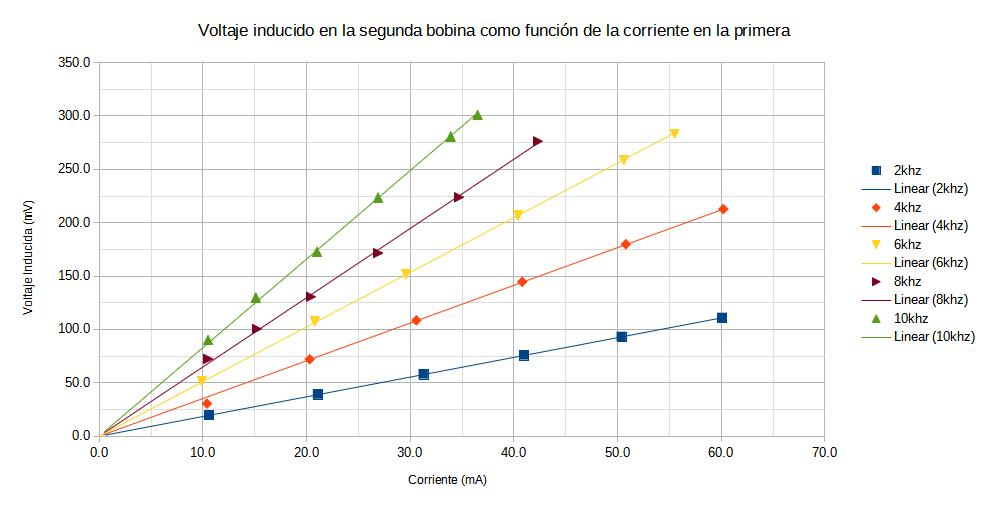
\includegraphics[width=\textwidth]{G12.jpg}

Si se hace la regresión lineal, se obtienen los siguientes valores para $k$ para los distintos valores de $f$:

\begin{table}[h!]
    \title{\textbf{Valores de las pendientes para diferentes valores de la frecuencia.}}
    \centering
    \begin{tabular}{|l|l|}
    \hline
        $f(Hz)$ & $k(\Omega)$\\\hline
        2000 & 1.84 \\ \hline
        4000 & 3.62 \\ \hline
        6000 & 5.08 \\ \hline
        8000 & 6.41 \\ \hline
        10000 & 8.10 \\ \hline
    \end{tabular}
\end{table}
\begin{center}
    \textit{Primaria: bobina 1$(\Phi = 12.5cm)$. Secundaria: bobina 3$(\Phi = 3.2cm)$}
\end{center}

Finalmente, se puede hacer un regresión lineal aquí y dividirla por $2\pi$, obteniendo el coeficiente de inducción mútua:

$$M_{12} =  1.22\cdot 10^{-4} H$$

De donde podemos obtener finalmente la permeabilidad magnética por la relación $(1)$:

$$\mu_0 = \frac{4M_{12} l_1}{N_1 N_2 \pi \Phi^2_2} = 1.25668 \cdot 10^{-6}$$

Y, considerando el número correcto de cifras significativas, tenemos que:

\begin{tcolorbox}
    \begin{equation}
        \mu_0 = 1.26 \cdot 10^{-6}
    \end{equation}
\end{tcolorbox}

Un resultado increíblemente próximo del teórico, $\mu_0 =  4\pi \cdot 10^{-7} = 12.56637\cdot 10^{-6}$, exactamente igual a el para las cifras significativas consideradas, o sea, se tiene que ele error relativo de este experimento fue de $0\%$.
\subsection{Comprobación de la simetría del coeficiente de inducción mutua}
Si se intercambiaran la bobina interior y la bobina interior, el resultado del coeficiente de inducción mútua debería ser igual al obtenido anteriormente. Esto es, el coeficiente es simétrico\footnote{\cite[322]{Griffiths}}, $M_{12} = M_{21}$. En este apartado, se desea verificar este hecho, haciendo la bobina 2 la primária y la 1 la secundaria.

Como esté valor no será utilizado para calcular $\mu_0$, se puede calcularlo de forma menos precisa, utilizando solamente la ecuación para $M$:

$$M_{21} = \frac{V_e}{2\pi f I_e}$$

De esta manera, tenemos que:
\begin{table}[h!]
    \title{\textbf{Valores de frecuencia, corriente y voltaje inducido}}
    \centering
    \begin{tabular}{|l|l|l|l|}
    \hline
        $f(Hz)$ & $I_e (mA)$ & $V_e (mV)$ & $M_{21}(H)$ \\ \hline
        2010 & 34.1 & 74.4 & $1.73\cdot 10^{-4}$ \\ \hline
        4120 & 33.9 & 150.2 & $1.71\cdot 10^{-4}$ \\ \hline
        6320 & 33.7 & 226.1 & $1.69\cdot 10^{-4}$ \\ \hline
        8000 & 33.5 & 281.8 & $1.67\cdot 10^{-4}$ \\ \hline
        9700 & 33.2 & 335.4 & $1.66\cdot 10^{-4}$ \\ \hline
    \end{tabular}
\end{table}
\begin{center}
    \textit{Primaria: bobina 2$(\Phi = 3.2cm)$. Secundaria: bobina 1$(\Phi = 12.5cm)$}
\end{center}
De donde podemos hacer la média de los valores de $M_{21}$, que nos indica un valor de $M_{21} = 1.69 \cdot 10^-4$, valor extremadamente dispar al de $M_{12}$. De esta manera, se puede asumir, sea por haber accidentalmente desplazado la bobina para un lado u otro o por haber conectado mal un cable, que hubo alguna fuente de error no considerada que llevo a tal equívoco. 
\subsection{Cálculo de $\mu_0$ a partir del coeficiente de inducción mutua entre las bobinas 1 y 3}
La ecuación $(1)$, en su derivación, asume que el campo magnético en el interior de la bobina más grande es uniforme. Esta aproximación es solamente válida para $l \ll l_1$, de manera que, si se tiene una bobina con longitud mayor que la de la bobina 2, se espera que produzca un resultado más impreciso de $\mu_0$. 

De esta manera, se repite el procedimiento de $3.1$ con otra bobina con $l$ mayor que la 2, la 3:

\begin{center}
    \textbf{Datos experimentales de la intensidad y tensión para diferentes valores de la frecuencia}
\end{center}

\begin{table}[h!]
    \hskip-1.5cm
    \begin{tabular}{|l|l|l|l|l|l|l|l|l|l|}
        \hline
    \multicolumn{2}{|c|}{f=2kHz} &\multicolumn{2}{|c|}{f=4kHz} &\multicolumn{2}{|c|}{f=6kHz} &\multicolumn{2}{|c|}{f=8kHz} &\multicolumn{2}{|c|}{f=10kHz}  \\ \hline
        $I_{e}(mA)$ & $V_e(mV)$ & $I_{e}(mA)$ & $V_e(mV)$ &$I_{e}(mA)$ & $V_e(mV)$ &$I_{e}(mA)$ & $V_e(mV)$&$I_{e}(mA)$ & $V_e(mV)$ \\ \hline
        13.0 & 84.9 & 11.4 & 118.4 & 11.5 & 198.4 & 10.2 & 237.0 & 9.5 & 268.7 \\ \hline
        19.1 & 123.1 & 21.4 & 236.5 & 16.7 & 282.9 & 15.2 & 338.8 & 13.6 & 374.5 \\ \hline
        24.5 & 157.9 & 28.8 & 317.4 & 23.9 & 403.9 & 18.2 & 404.9 & 17.6 & 481.8 \\ \hline
        30.2 & 194.0 & 33.6 & 369.3 & 30.2 & 514.0 & 21.2 & 468.7 & 21.1 & 578.0 \\ \hline
        37.1 & 237.9 & 37.6 & 413.8 & 34.3 & 583.0 & 23.8 & 531.0 & 24.7 & 675.0 \\ \hline
        44.2 & 283.0 & 41.0 & 450.9 & 41.3 & 701.0 & 27.3 & 608.0 & 30.5 & 831.0 \\ \hline
    \end{tabular}
\end{table}

\begin{center}
    \textit{Primaria: bobina 1$(\Phi = 12.5cm)$. Secundaria: bobina 3$(\Phi = 5.1cm)$}
\end{center}
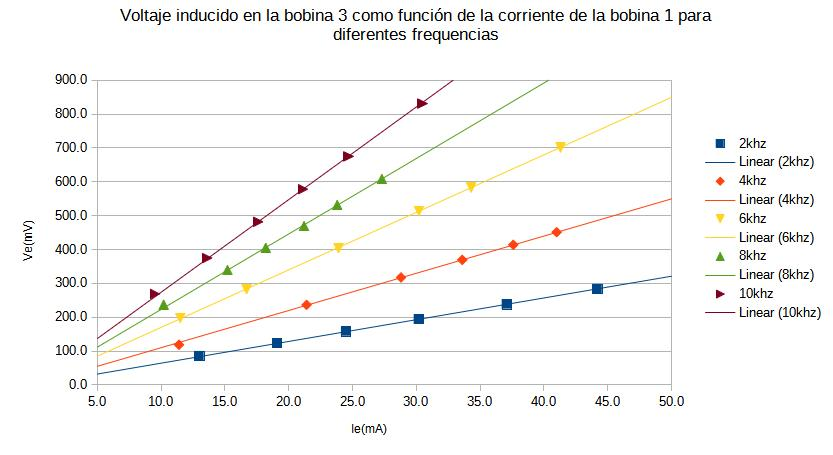
\includegraphics[width=\textwidth]{G13.jpg}
De donde se puede utilizar el mismo procedimiento de antes para adquirir $M_{13}$ y, consecuentemente, $\mu_0$. Se hacen las primeras regresiones lineales:
\begin{table}[h!]
    \title{\textbf{Valores de las pendientes para diferentes valores de la frecuencia.}}
    \centering
    \begin{tabular}{|l|l|}
    \hline
        $f(Hz)$ & $k(\Omega)$\\\hline
        2000 & 1.84 \\ \hline
        4000 & 3.62 \\ \hline
        6000 & 5.08 \\ \hline
        8000 & 6.41 \\ \hline
        10000 & 8.10 \\ \hline
    \end{tabular}
\end{table}
\begin{center}
    \textit{Primaria: bobina 1$(\Phi = 12.5cm)$. Secundaria: bobina 3$(\Phi = 5.1cm)$}
\end{center}

Y, haciendo otra regresión lineal, obtenemos que:

$$M_{13} = 4.11 \cdot 10^{-4} H$$

Y, por fín, se tiene que:

$$\mu_0 = \frac{4 M_{13} l_1}{N_1 N_3  \pi \Phi_3^2} = 1.23379 \cdot 10^{-6}$$

O sea, 

\begin{tcolorbox}
    \begin{equation}
        \mu_0 = 1.23 \cdot 10^{-6}
    \end{equation}
\end{tcolorbox}

Un valor de $\mu_0$ que tiene $\delta = \frac{\mu_{0teorico}-\mu_0}{\mu_{0teorico}} = 0.016$ del valor teórico, o sea, un desvío de $1.6\%$ del teórico. De esta manera, se ilustra como una medida hecha con un solenoide con mayor longitud es más imprecisa que de uno con menor.
 
\subsection{Comprobación de la uniformidad del campo magnético en el interior de un solenoide}
Para verificar la uniformidad del campo magnético de manera cualitativa, se puede medir el voltaje inducido en diferentes puntos de la bobina para mismos valores de corriente y frecuencia. Variaciones del voltaje significan variaciones en el campo magnético. Entonces, se tiene que:
\begin{center}
    \textbf{Valores de la voltaje inducida para diferentes posiciones en la bobina.}
\end{center}
\begin{table}[h!]
    \hskip-3.6cm
    \begin{tabular}{|l|l|l|l|l|l|l|l|l|l|l|l|l|l|l|l|l|l|}
    \hline
        $x(cm)$ & 1 & 4 & 7 & 10 & 13 & 16 & 19 & 22 & 25 & 28 & 31 & 34 & 37 & 40 & 43 & 46 & 49 \\ \hline
        $V_e(V)$ & 0.08 & 0.09 & 0.12 & 0.13 & 0.14 & 0.13 & 0.13 & 0.13 & 0.14 & 0.14 & 0.13 & 0.14 & 0.14 & 0.13 & 0.12 & 0.1 & 0.09 \\ \hline
    \end{tabular}
\end{table}

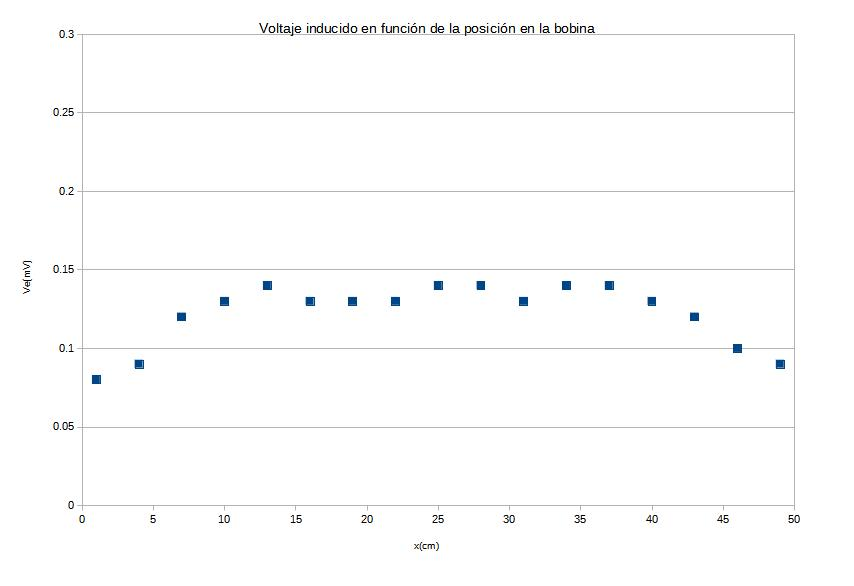
\includegraphics[width=\textwidth]{final.jpg}
O sea, el campo magnético es esencialmente constante en el intervalo de $10-40cm$.

\section{Conclusiones y Discusión}
Todos los resultados obtenidos están en completa concordancia con la bibliografía, a parte del coeficiente $M_{21}$, que debería verificar simetría con el $M_{21}$ pero no lo hace. 

Como era de se esperar, la precisión en el primero experimento, con la bobina de menor longitud de bobina, és más alta que en el segundo. Eso se explica por la aproximación de la uniformidad del campo empeorarse más allá de una longitud de $30cm$(región en que se puede considerar uniforme).

\printbibliography
\end{document}
